Quantitative evaluation constitutes the most critical part of this study in terms of measuring maintainability. As a part of this study, many other academic works on the measurement of maintainability in Android and software engineering were examined. The purpose of these reviews is to find the most appropriate maintainability measurement metrics. Various metrics can be used to evaluate object-oriented software systems in terms of quality and maintainability. The most popular of these metrics are detailed in Barak et al., (2012) \cite{33}. As a result of this examination, it was seen that the concepts of complexity, cohesion and coupling were emphasised in many studies, and it was concluded that the measurements made based on these concepts would be more efficient when measuring maintainability. The effects of these concepts on maintainability have been mentioned in the second chapter, and detailed studies in this field have been referred to. Studies have shown that results retrieved from evaluating these concepts proved to define the level of maintainability \cite{33}.

The definition of complexity in software engineering is the difficulty to understand the interactions between the parts of a software system. Higher levels of complexity in software increase the risk of accidentally preventing interactions, increasing the chance of introducing bugs when making changes, thus decreasing maintainability. High coupling between classes also causes complexity when maintaining the software. Changes done in a class reflect the dependent class due to the dependency relationship of the classes. Thus, the software system becomes challenging to maintain. In software engineering, cohesion is how well the methods of a class are related to each other. While the classes' relationship is desired to be loosely coupled, their methods and data fields are desired to be related. Lack of cohesion threatens modularity and software maintenance. 
\begin{figure}[ht!]
    \centering
    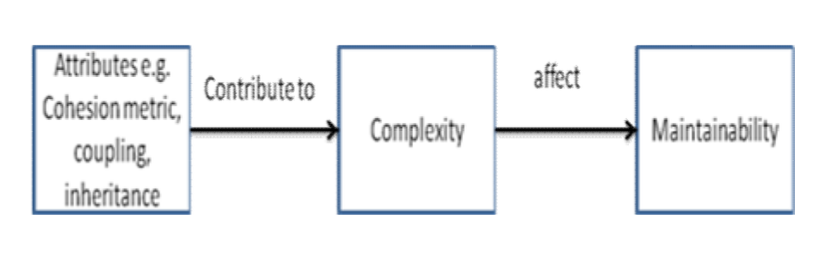
\includegraphics[scale=0.5]{figures/maintainability_factors.png}
    \caption{Relationship between cohesion, coupling, complexity and maintainability \protect\cite{33}}
    \label{fig:maintainability_factors}
\end{figure}

As can be seen, complexity, cohesion and coupling are in a tight relationship among themselves, and they all directly affect software maintainability. The figure below shows the relationship between maintainability, complexity, cohesion and coupling. Therefore, based on this result, research was done on measuring the concepts of complexity, cohesion and coupling effectively, and the most suitable metrics for measurement were determined. As a result of this research, five metrics that will enable an object-oriented software system to be evaluated effectively in terms of complexity, cohesion and coupling have been determined. While selecting these metrics, priority has been given to metrics that can handle a software system as a whole in the areas of complexity, cohesion and coupling. This enables the system to be evaluated in terms of maintainability in the most effective way. To emphasise again, although these metrics are used in measuring complexity, cohesion and coupling, they allow maintainability to be measured directly due to the tight relationship between these concepts and software maintainability. These metrics and their intended use are listed below. 
\begin{itemize}
    \item \textbf{Weighted Method Count (WMC):} This metric is used to measure object-oriented software systems’ complexity. WMC represents a class's cyclomatic complexity, also known as McCabe complexity \cite{35}. It, therefore, portrays the complexity of a class as a whole, and this measure can be used to indicate the maintainability level of the class. The number of methods and complexity can be used to divine maintaining effort. If the number of methods is high, that class is described as domain-specific and is less reusable. Also, such classes tend to be prone to change and defects.
    \item \textbf{Depth of Inheritance Tree (DIT):} This is another metric to measure software complexity. Inheritance increases software reusability; however, one side can create complexity by possibly violating encapsulation since the subclass needs to access the superclass. Furthermore, changes made during maintenance might increase the inheritance tree's depths by adding more children. Therefore, by assessing the inheritance tree available in the product, it is easy to predict how much effort needed to make it stable \cite{33}. It is harder to predict its behaviour if the tree depth is high, and this causes maintenance issues.
    \item \textbf{Number of Children (NOC):} NOC measures the number of descendants of a class, and it is used to measure the coupling level for the corresponding class. NCO also indicates the reusability level of a software system. It is assumed that the number of child classes and the maintainer's responsibility to maintain the children's behaviour are directly proportional. If the NOC level is high, it is harder to maintain and modify the class \cite{36}.
    \item \textbf{Coupling Between Object Classes (CBO):} This metric calculates the number of connections to other classes from a particular class, and it is used to measure coupling. A class is considered coupled if it depends on another class to get its work done \cite{34}. CBO metric is related to the reusability of the class. High coupling makes the code more difficult to maintain because changes in other classes can also affect that class. Therefore these classes are less reusable and less maintainable.
    \item \textbf{Lack of Cohesion of Methods (LCOM):} This metric is used to determine how class methods are related to each other, and it is applied to evaluate cohesion. Cohesion promotes the maintainability of the software systems. High cohesion for a class meant the class is understandable, maintainable and easy to modify \cite{33}.
\end{itemize}

Apart from the above metrics, many other metrics can measure quality and maintainability in object-oriented software systems. The most well-known of these metrics are the Line of Code (LOC) and Halstead Effort metrics. Studies conducted using these metrics in Android, and other software development fields were examined within this study's scope. The methods related to size were not preferred because they were too classical, and they do not give very effective results on maintainability. Halstead complexity metrics were not preferred because they concentrated more on the complexity of classes and methods. Regarding the use of these metrics, Prabowo's work on Android apps' maintainability can be examined \cite{19}. Instead, metrics that facilitate evaluating the quality and maintainability of software systems as a whole were preferred.

After determining the metrics to be used, research has been conducted on how these metrics will be applied. As a result of the research, it has been concluded that metrics can be applied manually or with a tool's help. Since manual implementation will take more time and is prone to error, it has been decided to apply metrics with a reliable tool. Later, a search was done for a static code analysis tool to work with Android Studio and Kotlin programming languages and support the selected metrics. During the research, the CodeMR static code analysis tool drew attention. CodeMR is a powerful software quality tool that is integrated with IDEs and supports multiple programming languages. Java, Scala, Kotlin and C++ \footnote{\url{https://www.codemr.co.uk}}. The tool provides an understanding of software quality through its metrics to measure coupling, complexity, cohesion and size. These metrics are often affected by various code characteristics, making them promising for evaluating software maintainability.  Besides, the tool provides a visualisation centric approach and generates detailed reports supported by different visualisation options. In this way, it facilitates the application of metrics and makes the results more understandable with detailed reports and advanced visualisation techniques. The tool can also be installed as a plugin in Android Studio and is very easy to use. Apart from that, the tool also makes it possible to measure with many other metrics. The complete list of metrics and other features that the tool offers can be accessed via the tool's documentation. Finally, 2 academic studies conducted using this tool were examined before the tool was started to be used, and information about the tool operation was obtained\cite{38}\cite{39}. Finally, the CodeMR static code analysis tool has been chosen to be used in this study due to the support of Kotlin, its ability to be installed as an add-on to Android Studio, its support for selected metrics, and its advanced visualisation and reporting mechanisms. After this decision, communication was established with the CodeMR team, and a free license was obtained to be used in academic studies. 

The use of metrics (CodeMR static code analysis tool) to measure the impact of technologies, methods and principles used by the Mooncascade Android team on maintainability was realised as described following. First of all, a pilot project where metrics can be applied has been determined. While determining the pilot project, the priority was to find a project with an old version developed using outdated technologies, methods, and a weakly structured architecture. However, this project should also have had a new version developed with current technologies and methods mentioned in this study. Thus, using the metrics mentioned above, the impact of the team's current methods on maintainability could be measured. Because of Mooncascade's wide range of realised and ongoing projects, finding a project that met these conditions was possible. Although the full content cannot be published due to the privacy principles and confidentiality, it was possible to apply quantitative evaluation by applying selected metrics to the available features of the old (actively in use) and new codebases (still under development) of an Android application. In this way, it was aimed to evaluate the effects of the methods, principles and technologies used by the Mooncascade Android team on maintainability at the maximum level effectively. Detailed information and evaluation of the results will be shared in section \ref{section:5}.